\documentclass[pdftex,12pt,a4paper]{report}

\usepackage[utf8]{inputenc}
\usepackage[T1]{fontenc}
\usepackage[francais]{babel}
\usepackage{setspace}
\usepackage[top=2.5cm,bottom=2.5cm,right=3cm,left=3cm]{geometry}
\usepackage{parskip}

\usepackage{hyperref}
\usepackage{color}

\usepackage{calc}
\usepackage{pseudocode}

\usepackage[pdftex]{graphicx}
\usepackage{float}
\usepackage{caption}
\usepackage{fancybox}

\usepackage{caption}
\captionsetup{figurewithin=none}  
\captionsetup{tablewithin=none}

\AddThinSpaceBeforeFootnotes

\FrenchFootnotes

\newcommand{\HRule}{\rule{\linewidth}{1mm}}

\setlength{\parskip}{1mm}

\begin{document}

\begin{titlepage}
  \begin{sffamily}
  \begin{center}

    % Upper part of the page. The '~' is needed because \\
    % only works if a paragraph has started.
    
\includegraphics[scale=0.6]{./img/univ-lille1.png}~\\[1.5cm]
    
    \textsc{\Large Master INFORMATIQUE}\\[0.5cm]
    
    \textsc{\Large Mention INFORMATIQUE}\\[2cm]

    \textsc{\LARGE Rapport de ProJet Encadré}\\[2cm]

    % Title
    \HRule \\[0.4cm]
    { \huge \bfseries Analyse de Comportements avec Twitter\\[0.4cm] }

   \vfill

    % Author and supervisor
    \begin{minipage}{0.4\textwidth}
      \begin{flushleft} \large
        Antonin \textsc{Carette}\\
        Alexandre \textsc{Verkyndt}\\
      \end{flushleft}
    \end{minipage}
    
    \vfill

    % Bottom of the page
    {\large Promo 2014/2015}

  \end{center}
  \end{sffamily}
\end{titlepage}

\begin{spacing}{1.2}

\tableofcontents

\chapter*{Introduction}

\addcontentsline{toc}{chapter}{Introduction} 

\section{Problèmatique}

Le but de ce projet était de réaliser une application permettant d'analyser les comportements de tweets contenus dans l'application Twitter (en particulier, l'analyse de sentiments), via l'utilisation de son interface de programmation.\\
L'analyse de comportements sera étudié via différents algorithmes de classification (ou modèle), utilisant ou non une base d'apprentissage : le modèle basique (basé sur des dictionnaires), le modèle KNN et enfin le modèle Bayesien.

\section{Interface de programmation Twitter}

Pour ce projet, nous allons utiliser l'interface de programmation\footnote{Une interface de programmation est aussi appelée "API".} de Twitter.\\
Cette API nous permettra de récupérer les tweets voulus, sur un sujet donné, ainsi que toutes les informations suivantes : l'ID du tweet, l'émetteur, s'il s'agit d'un tweet original ou s'il s'agit d'un \textit{retweet}\footnote{Un \textit{retweet} est un tweet partagé - il n'est alors en aucun cas original.}.\\
Aussi, nous allons utiliser cette interface via la librairie Java \textit{Twitter4J}, dans sa version stable. En effet, cette librairie (à jour en fonction des mises à jour de l'interface de programmation) Java nous permettra d'accéder facilement aux tweets recueillis ainsi qu'aux informations du tweet, via des classes et des méthodes Java programmées.

\chapter{Présentation du logiciel}

\section{Généralités}

Ce programme a été écrit avec Java et Swing, pour la partie Interface Utilisateur.
\\
Suite à l'utilisation de fonctions avancées telles que le \textit{switch} sur une chaîne de caractères, ou le \textit{cast} des \textit{JComboBox}\footnote{Liste d'options graphique, en Java.}, ce programme n'est compatible qu'avec une machine virtuelle Java de version 7 ou plus.

\subsection{Titre et logo}

Notre logiciel se nomme \textit{BehAnTweet}\footnote{La documentation développeur du logiciel est présente dans le répertoire \textit{\textbf{doc}}, à partir de la racine du projet.}. Le nom du logiciel se réfère à la phrase anglaise "Behavior Analysis of a Tweet", littéralement "Analyse de Comportement d'un Tweet", qui est le sujet de notre projet encadré.
\\
Le logo du logiciel est, quant à lui, une référence à \textit{Bahamut}\footnote{Un poisson (ou serpent géant), présent dans la mythologie Arabe.}, déposé sous licence libre.

\subsection{Logiciels de versionning utilisés}

\textit{Git} a été utilisé comme logiciel de versionning principal pour la gestion du projet, dû à sa simplicité d'emploi par rapport à \textit{svn} mais aussi à l'utilisation faite de ce logiciel depuis plusieurs mois sur d'autres projets et à l'application web interactive \textit{Github}\footnote{\url{https://github.com/WebTogz/BehAnTweet}}.\\
\textit{Svn} a lui été utilisé pour transmettre la version principale du logiciel sur les serveurs de l'Université\footnote{\textbf{Serveur} : svn-etu.fil.univ-lille1.fr; \textbf{Projet} : pje14-15-carette.}, toutes les 3 semaines, afin de pouvoir visualiser l'avancement du projet régulièrement.
\\
Une utilisation poussée de \textit{Git} a été effectuée : gestion des commits en binôme, commits de chaque petite partie de code, création et gestion de plusieurs branches, merge avec la branche \textit{origin}, etc...

\section{Description de l'architecture de l'application}

Nous avons utilisé principalement le modèle \textbf{MVC} (pour Modèle - Vue - Contrôleur) pour notre projet.\\
Ce modèle, très connu pour le développement logiciel, est destiné à répondre aux besoins des applications interactives, en séparant les problématiques liées aux différents composants au sein de leur architecture respective.\\
Aussi, le gros bénéfice de ce patron est qu'il permet facilement l'évolution de l'application par la suite, via l'ajout de classes dans les packages spécifiques suivants: \textbf{Controler}, \textbf{Model}, \textbf{View}.

\subsection{Packaging}

\subsubsection{Controler}

Le contrôleur prend en charge la gestion des événements de synchronisation pour mettre à jour la vue ou le modèle, et les synchroniser. Il analyse la requête du client et se contentera alors de renvoyer la vue correspondant à la demande, en fonction du modèle appelé. Aussi, il est important de savoir que le contrôleur n'effectue aucun traitement, et ne modifie aucunement les données !
\\
Il était ainsi nécessaire d'implémenter le patron \textbf{Observable/Observeur}, afin de pouvoir un Observer (objet qui observe) qu'une modification a été apporté sur un Observable (objet observé par un Observer).

\subsubsection{Model}

Le modèle est le coeur algorithmique de l'application - il gère le traitement des données, la mise à jour des vues mais aussi les interactions avec la base de données.
\\
Le package Model contiendra tous les modèles de l'application - chaque modèle (à part la base Model.java) contiendra sa propre implémentation d'un algorithme de classification (Dictionnaire, KNN, Bayes).

\subsubsection{View}

La vue est le coeur de l'intéraction avec l'application.
\\
Elle détient plusieurs tâches à effectuer:
\begin{itemize}
\item{la première est de présenter les résultats renvoyés par le modèle,}
\item{la seconde est de recevoir l'action de l'utilisateur - via la manipulation de boutons, objets cliquables, etc...}
\end{itemize}
Toutes ces tâches, une fois finalisées, seront renvoyées au Contrôleur de l'application afin de pouvoir être traitées par le modèle.

\section{Interface graphique}

Nous avons pensé avant tout à une utilisation simple du logiciel, reposant sur une seule fenêtre. Cette fenêtre contiendra tous les paramètres pouvant être manipulés par l'utilisateur (le nombre de tweets à recueillir, l'algorithme utilisé et ses spécifications), une barre de recherche concernant un sujet donné, et enfin un grand espace dédié à la liste des tweets recueillis et de leur classification par l'algorithme choisi.

\subsection{Capture d'écran}

Vous trouverez ci-dessous l'écran principal de l'application. Il est constitué en 4 grandes parties, pouvant être divisées chacune à leur tour.
\begin{itemize}
\item{\textbf{encart de recherche (1)} : contient la barre de recherche de tweet, le bouton de recherche "Search", le bouton de nettoyage du fichier temporaire tweet\_clean.csv "Clean", et le bouton de validation "Validate"\footnote{Le bouton "Validate" permet la sauvegarde des tweets recueillis après vérification des comportements, dans un fichier temporaire.},}
\item{\textbf{encart de visualisation (2)} : visualisation des tweets\footnote{Un exemple de tweet peut être visualisé en \textbf{3} - nous pouvons ainsi voir la classification obtenue du tweet par le classifieur utilisé (ici le classifieur par mot-clef), ainsi que le corps du tweet sur la droite.} recueillis,}
\item{\textbf{encart statistiques (4)} : visualisation des statistiques concernant la dernière recherche effectuée - elle pourra s'effectuer par visualisation des pourcentages de tweets classifiés, ou alors par visualisation du camembert, donnant une réponse visuelle immédiate quant à l'ensemble des tweets classifiés (juste en dessous de sa légende),}
\item{\textbf{encart de paramètres (5)} : ce sont les paramètres ajustables de l'application - cet encart contient la modification du nombre de tweets à recueillir, la méthode de classification à utiliser ainsi que les paramètres Bayèsiens à prendre en compte.}
\end{itemize}

\rotatebox{90}{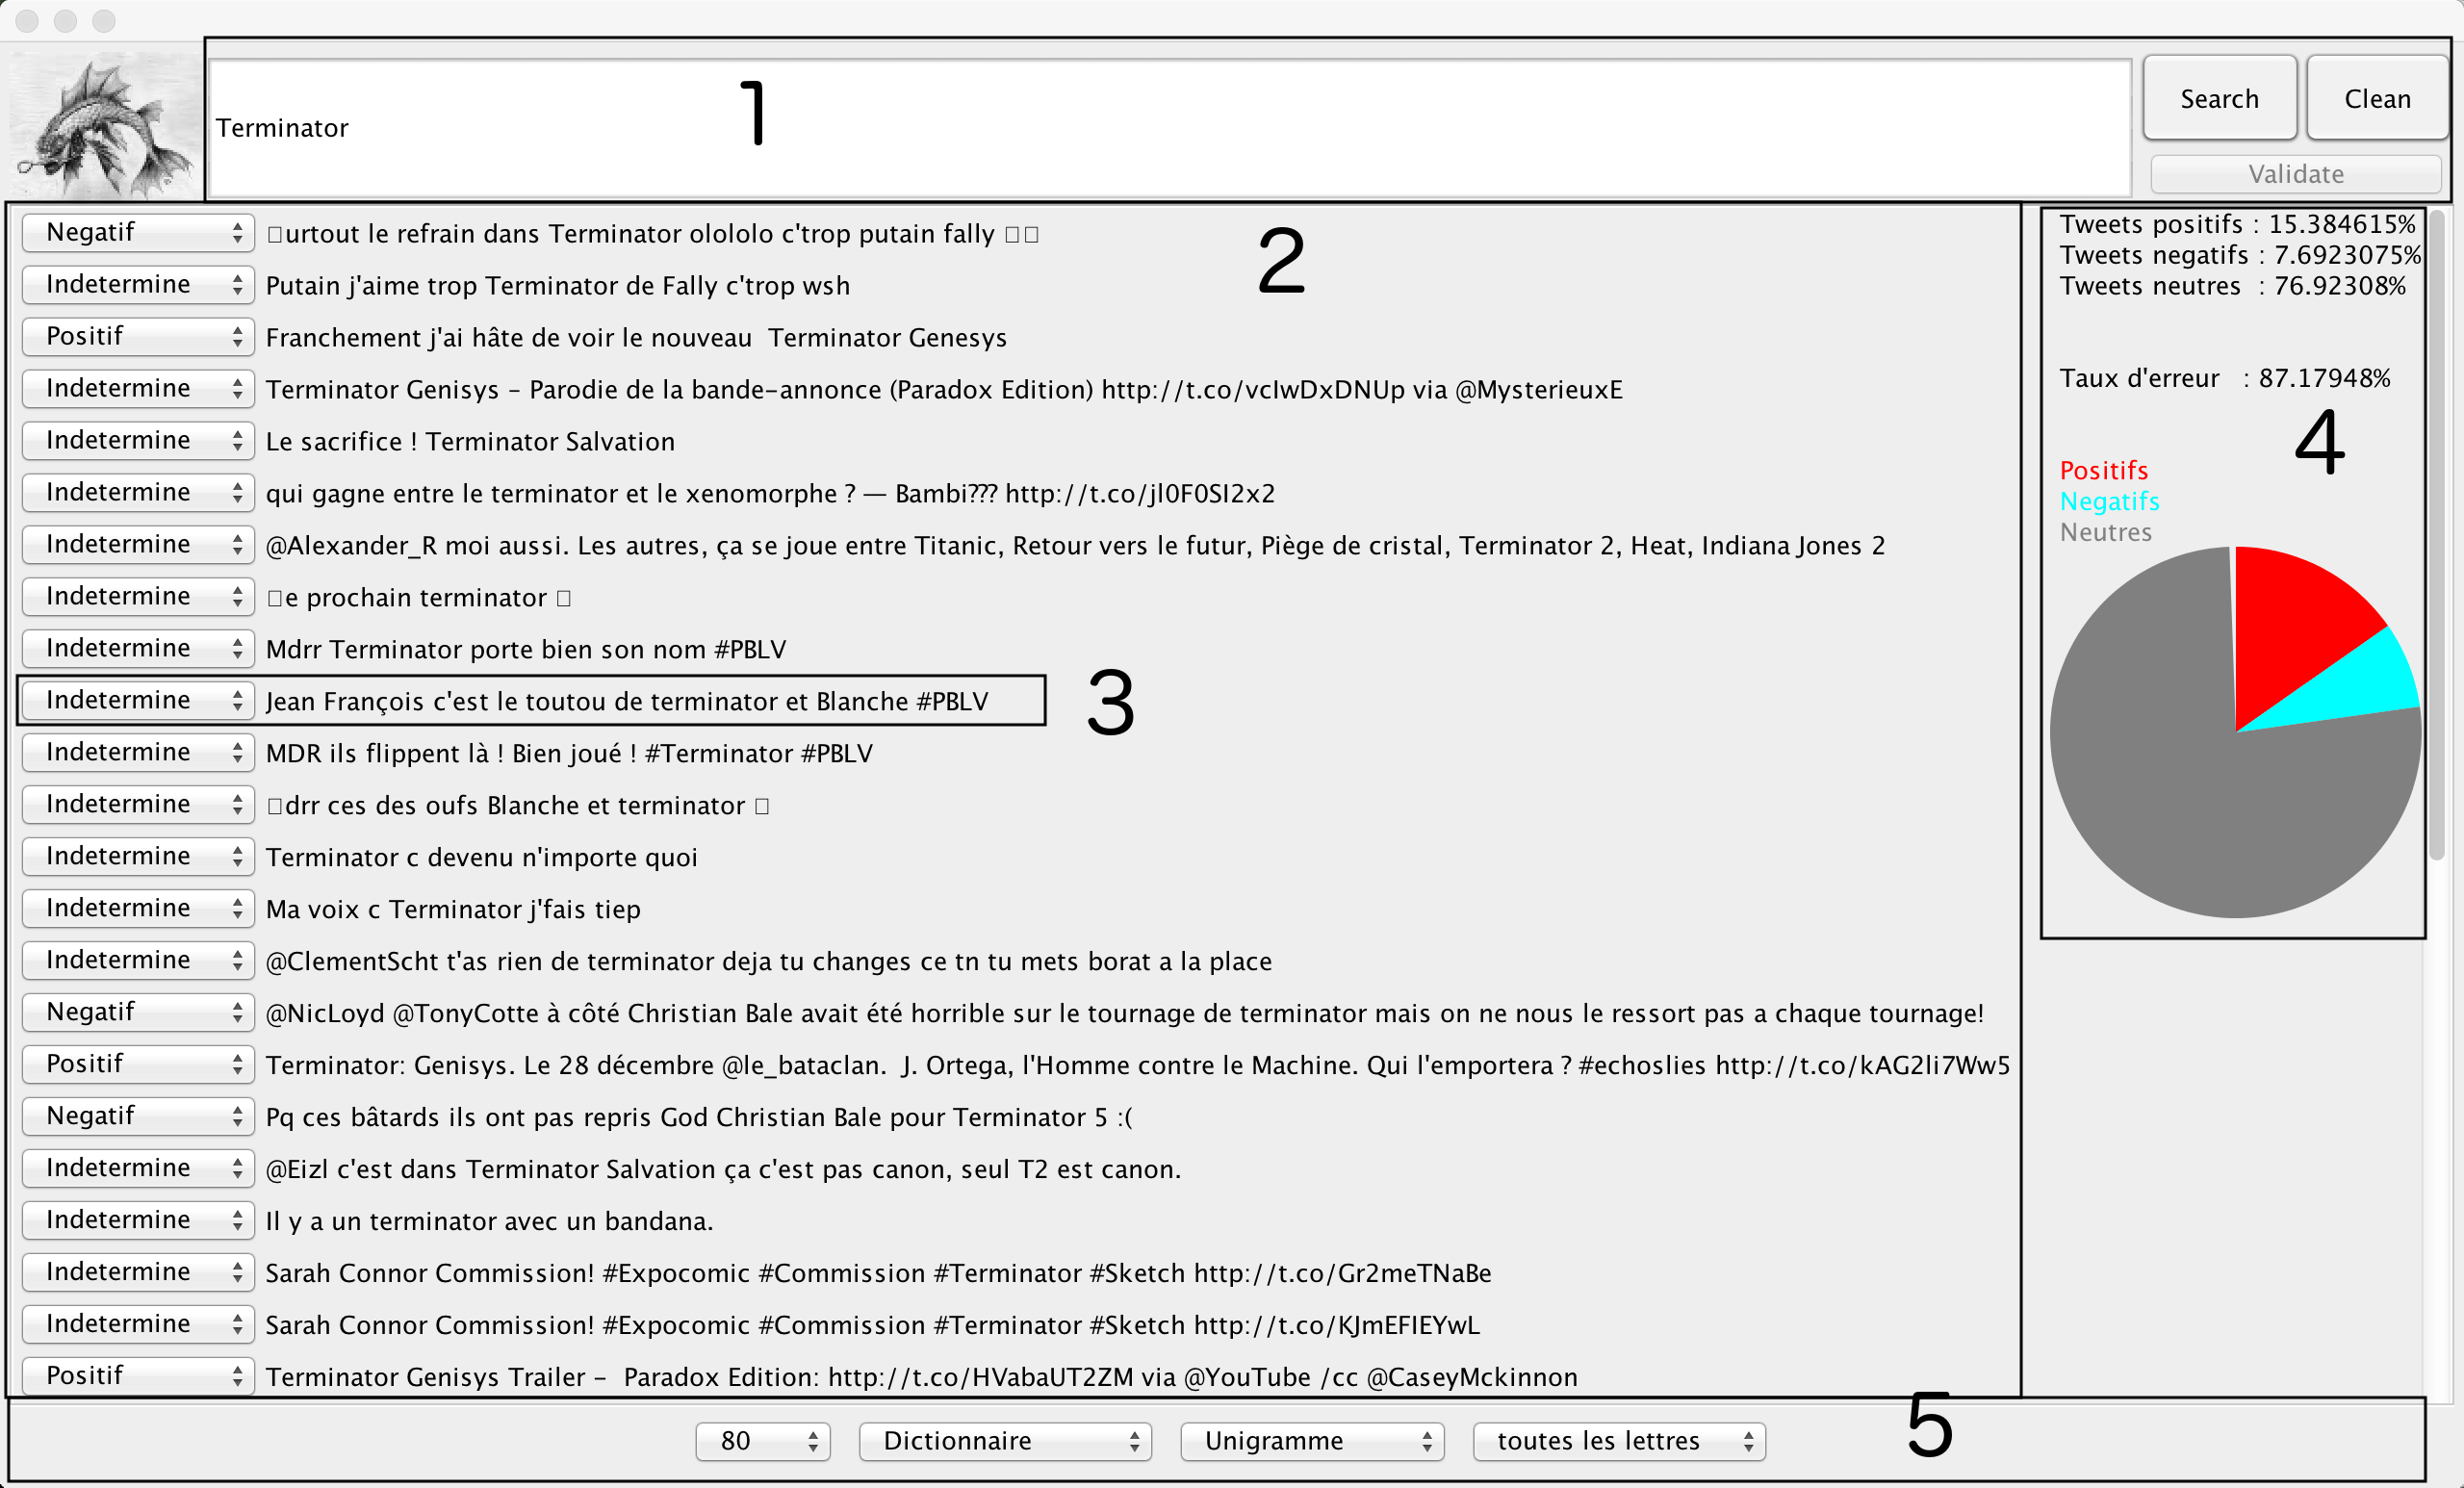
\includegraphics[scale=0.53]{img/BehAnTweet_main.png}}

\subsection{Manuel d'utilisation}

\subsubsection{Comment modifier les paramètres réseaux de l'application?}

Ouvrez le fichier \textit{twitter4j.properties}.
\\
Recherchez les deux lignes situées sous le commentaire : //PROXY.
\\
\\
\underline{Si vous vous trouvez sur l'Université Lille1}, veuillez entrer les propriétés proxy : 
\\	http.proxyHost=cache-etu.univ-lille1.fr
\\	http.proxyPort=3128
\\
\\
\underline{Si vous ne vous trouvez pas sur sur l'Université Lille1}, vous pouvez désactiver les propriétés proxy en commentant les lignes précédentes.

\subsubsection{Comment modifier le nombre de tweets recueillis pour une requête?}

Dans l'encart des paramètres, cliquez sur le bouton "20" - cela signifie que le nombre de tweets maximal affiché est de 20.
\\
Cliquez alors sur la nouvelle valeur que vous voulez prendre en compte.

\subsubsection{Comment modifier la méthode de classification pour une requête?}

Dans l'encart des paramètres, cliquez sur le bouton "Dictionnaire", et choisissez alors votre méthode de classification.
\\
Si vous choisissez la méthode Bayes Fréquence, choisissez alors le nombre de grammes que vous voulez utiliser, et enfin le "type" de mots que vous voulez comparer - avec le nombre de lettres par mot.

\subsubsection{Comment effectuer une requête?}

Vous pouvez effectuer une recherche en tapant votre requête dans la barre de recherche de tweet. Après cela, vous pouvez choisir dans l'encart de paramètres le nombre de tweets maximal à recueillir pour cette requête, ainsi que la méthode de classification demandée.
\\
Après le choix des paramètres, cliquez sur le bouton "Search" afin de lancer votre requête, via \textit{Twitter4J} et l'API Twitter. Vous obtiendrez alors dans l'encart de visualisation, quelques secondes après, un ensemble de tweets recueillis et en lien à cette recherche.

\subsubsection{Comment modifier la classification d'un ou de plusieurs résultat(s) de requêtes?}

Après une requête, vous pouvez remarquer dans l'encart de visualisation que, via la méthode de classification choisie, une classification est déjà établie - à gauche du tweet.
\\
Si la classification d'un tweet ne vous plaît pas, vous pouvez la modifier en cliquant sur la classification du tweet. Vous pouvez alors choisir la classification qui vous plaît en cliquant sur celle choisie.
\\
Vous pourrez alors constater que votre demande a bien été prise en compte, via le changement de la classification dans l'encart de visualisation.

\subsubsection{Comment enregistrer les résultats d'une requête dans la base d'apprentissage?}

Une fois les classifications de chaque tweet analysées, vous pouvez enregistrer celles-ci dans un fichier CSV temporaire (tweet\_clean.csv), en cliquant sur le bouton "Validate", présent dans l'encart de recherche. Une fois cliqué, le bouton devient gris - il ne vous ai plus possible de valider une seconde fois ces mêmes classifications.
\\
Pour enregistrer les tweets recueillis dans la base d'apprentissage, il suffit juste d'ouvrir le fichier base\_apprentissage.csv, et de copier/coller tous les tweets que vous voulez enregistrer dans celle-ci.
\\
L'avantage de cette solution est de permettre à l'utilisateur de choisir exactement le ou les tweet(s) qu'il veut sauvegarder, et le ou les tweet(s) qu'il veut ignorer.
\\
\\
\textbf{ATTENTION} : si vous voulez enregistrer les tweets nettoyés dans le fichier tweet\_clean.csv sans tenir compte des résultats précédents sauvés dans ce même fichier, il sera nécessaire de cliquer sur le bouton "Clean" - qui nettoiera le fichier tweet\_clean.csv - avant de cliquer sur "Validate".

\chapter{Algorithmes de classification}

Pour l'analyse de tweets, divers algorithmes de classification ont été utilisés.\\
Voici la liste des algorithmes de classification utilisés.

\section{Dictionnaire}

La méthode \textbf{Dictionnaire} (ou encore par \textbf{mot-clef}) a été l'algorithme le plus facile à programmer.\\
En effet, il consiste dans un premier temps à obtenir une liste de mots positifs et négatifs. Chaque tweet recueilli sera découpé en mots, et chaque mot sera confondu avec les deux listes - aussi, le tweet partira avec un score entier nul. Si un des mots du tweet est reconnu dans la liste de mots positifs, on diminuera son score - à contrario, si ce mot est reconnu dans la liste de mots négatifs, on augmentera son score. Ainsi, chaque mot du tweet est un mot-clef à reconnaître.
\\
\\
Finalement, on obtiendra pour chaque tweet un score, somme des scores de chaque mot appartenant à celui-ci. Ce score décidera de la classification auquel appartient le tweet:
\begin{itemize}
\item{positif, si le score est négatif,}
\item{indéterminé, si le score est nul,}
\item{négatif, si le score est positif.}
\end{itemize}

\section{KNN}

La méthode \textbf{KNN}\footnote{Aussi appelé méthode des \textit{k} plus proches voisins.}, est une méthode d'apprentissage automatique basée sur des exemples contenus dans une base d'apprentissage.
On cherchera ici à trouver les \textit{k} plus proches tweets du tweet analysé, contenus dans la base d'apprentissage du projet\footnote{Cette base d'apprentissage consiste en la sauvegarde de tweets déjà analysés pour le comportement.}.
\\
\\
Pour chaque tweet, on aura un tableau de \textit{k} objets, contenant un couple (distance, tweet). On range ainsi les \textit{k} premiers tweets de la base d'apprentissage dans le tableau énoncé précédemment, les distances étant calculées entre le tweet à classifier et le tweet de la base d'apprentissage selon la formule suivante : \textbf{((nombreMotsTotal) - nombreMotsCommuns) / nombreMotsTotal}.
\\Pour les (\textit{k}+1) à \textit{n}\footnote{\textit{n} étant le nombre de tweets total contenus dans la base d'apprentissage.} tweets, on calculera à chaque fois la distance entre le tweet courant et le tweet à classifier. Si cette distance est inférieure à la plus grande distance contenue dans le tableau des \textit{k} objets, on remplacera alors cet objet par la nouvelle distance ainsi que le tweet courant associé à celle-ci.
\\
\\
Une fois cette étape faite, il nous restera à définir le comportement du tweet à classifier - pour cela, on comptera combien il y a de tweets positifs issus de la base d'apprentissage, de même pour les tweets négatifs et indéterminés. Le score le plus élevé parmi les 3 sera l'avis décisif pour le tweet à classifier.

\section{Bayes}

La \textbf{classification Bayésienne} est, quant à elle, basée sur les probabilités conditionnelle et la règle de Bayes. Aussi, on se servira d'une base d'apprentissage, car nous avons besoin de connaissances afin de pouvoir classifier les tweets recueillis.\\
Pour la méthode Bayès, nous utiliserons deux sous-méthodes de classification: \textit{Présence} et \textit{Fréquence}. Pour la classification par Fréquence, on estimera la probabilité d'occurence d'un événement, ce qui n'est pas pris en compte pour la classification par Présence.

\subsection{Présence}

On devra déterminer la classe la plus probable pour un tweet. Pour cela, on utilisera la règle de Bayes : P(\textit{c} | \textit{t}) = P(\textit{t} | \textit{c}) . P(\textit{c}) / P(\textit{t}), où \textit{c} est la classe d'un tweet (Positif, Négatif ou Indétermine), et \textit{t} le tweet à classifier.
\\
Dans cette sous-méthode, on ne se préoccupe pas du nombre d'occurrences des mots.

\subsection{Fréquence}

Dans cette sous-méthode, on prendra en compte le nombre d'occurrences d'un mot du tweet à classifié.
\\
On pourra considérer ici plusieurs combinaisons de mots:
\begin{itemize}
\item{uni-gramme,}
\item{bi-gramme.}
\end{itemize}
Par exemple, considérer "chef d'oeuvre" comme uni-gramme serai considérer le mot "chef" et le mot "oeuvre", indépendamment l'un de l'autre. À contrario, considérer ce même mot comme bi-gramme serai bien le considérer comme un seul mot.
\\
Aussi, on pourra considérer de calculer cette fréquence sur tous les mots du tweet, ou alors sur seulement des mots ayant un certain nombre de lettres pour ne pas être considérés comme des mots inutiles (comme "le", "la", "les", "de", "du", ...).
\\
Tout ceci pourra réduire les calculs (sans affecter le modèle de classifier), et marquer l'importance de certains mots ou certains groupes de mots. 

\chapter{Résultats de la classification}

Nous travaillerons sur un ensemble d'apprentissage basé sur le mot-clef "\textbf{Terminator}".
\\
La base d'apprentissage, elle, contient 173 tweets classifiés.

\section{Dictionnaire}

Cet algorithme, facile à implémenter, est malheureusement peu fiable mais aussi assez lent. En effet, il s'appuie sur deux dictionnaires : un dictionnaire positif et un négatif - cet algorithme ne s'appuie donc pas sur une base d'apprentissage. Surtout, il ne comptabilise pas les mots qui ne sont pas présents dans les deux dictionnaires, ce qui est n'est pas évident pour la conjugaison d'un verbe par exemple, ou alors lors d'une malencontreuse faute d'orthographe dans le mot...
\\
Aussi, l'algorithme est lent car, à chaque tweet, il doit regarder si chaque mot issu du dictionnaire positif est présent dans le tweet à analyser - de même pour le dictionnaire négatif.
\\
\\
\begin{tabular}{|l|c|c|r|}
  \hline
  \textbf{Tweets positifs} & \textbf{Tweets négatifs} & \textbf{Tweets indéterminés} & \textbf{Taux d'erreur}\\
  \hline
  15\% & 10\% & 75\% & 85\%\\
  \hline
\end{tabular}
\\
\\
Nous pouvons remarquer ici que la classification est majoritairement indéterminée (75\%) - en effet, il peut être difficile de trouver le mot exact dans le dictionnaire, et pouvoir ainsi classifier le tweet en fonction de la somme des scores de chaque mot. La classification positive et négative est presque équivalente - 15\% de tweets positifs et 10\% de tweets négatifs.

\section{KNN}

L'algorithme implémenté pour KNN se base sur une base d'apprentissage - à savoir un fichier CSV contenant tous les tweets sauvés et dont la classification de chaque tweet a été vérifié.
\\
Pour que la classification se fasse de façon optimale, il faut une base d'apprentissage rigoureuse mais aussi de taille très grande. De plus, il aurai fallu choisir \textit{k} de façon optimale aussi, ce qui n'a pas été effectué dans le cadre de ce projet.
\\
\\
\begin{tabular}{|l|c|c|r|}
  \hline
  \textbf{Tweets positifs} & \textbf{Tweets négatifs} & \textbf{Tweets indéterminés} & \textbf{Taux d'erreur}\\
  \hline
  25\% & 55\% & 20\% & 80\%\\
  \hline
\end{tabular}
\\
\\
En résultat de l'exploitation des résultats, nous pouvons observer que nous obtenons une majorité de tweets négatifs (55\%), un ordre de tweets positifs de l'ordre de 1/4 (25\%) ainsi que 20\% de tweets indéterminés, le tout pour un taux d'erreur de l'ordre de 80\%.
\\
Nous pouvons observer que cet algorithme KNN a travaillé pour classifier les tweets recueillis, et ne les a pas classer en majorité en indéterminé.

\section{Bayes}

Voici un tableau permettant de visualiser le taux d'erreur d'algorithmes de classification bayésienne, à savoir \textbf{Présence uni-gramme}, \textbf{bi-gramme} et \textbf{uni+bi-gramme}, mais aussi \textbf{Fréquence uni-gramme}, \textbf{bi-gramme} et \textbf{uni+bi-gramme}.
\\
\\
\begin{tabular}{|l|c|c|c|r|}
  \hline
  \textbf{Algorithme} & \textbf{Tweets pos.} & \textbf{Tweets nég.} & \textbf{Tweets indét.} & \textbf{Taux d'erreur}\\
  \hline
  Prés., uni & 21.05\% & 31.57\% & 47.37\% & 82.46\%\\
  Prés., bi & 0\% & 36.84\% & 63.16\% & \textbf{36.84}\% \\
  Prés., uni + bi & 0\% & 78.95\% & 21.05\% & 78.95\% \\
  Fréq., uni & 35\% & 0\% & 65\% & \textbf{41.67}\% \\
  Fréq., bi & 10\% & 0\% & 90\% & \textbf{33.33}\% \\
  Fréq., uni + bi & 20\% & 0\% & 80\% & 83.33\% \\
  \hline
\end{tabular}
\\
\\
Nous pouvons remarquer que la classification Bayésienne par présence bi-gramme est la plus précise (taux d'erreur de 36.84\% - aucun tweet positif mais 36.84\% de tweets négatifs et 63.16\% de tweets indéterminés) - à contrario, l'uni-gramme est celle ayant le plus grand pourcentage d'erreur (82.46\% en taux d'erreur - aucun tweet positif non plus, 78.95\% de tweets négatifs et 21.05\% de tweets indéterminés). Quant à l'unicité uni-gramme/bi-gramme, elle obtient un résultat compris entre les deux les précédents (78.95\%).
\\
Nous pouvons avoir une incompréhension lors de la vue des résultats quant à la classification Bayésienne par Fréquence - en effet, les résultats sont assez proches les uns des autres, sauf pour l'uni-gramme/bi-gramme (83.33\%) qui a un taux d'erreur bien plus élevé que l'uni-gramme (42.67\%) et le bi-gramme (33.33\%) indépendants l'un de l'autre. Ainsi, on pourra douter du bon calcul du taux d'erreur pour cette dernière. L'uni-gramme et le bi-gramme sont, à contrario, plus précis que ceux concernant la classification Bayésienne par Présence, et ne détient par de tweets négatifs (35\% de tweets positifs pour la Fréquence uni-gramme, 65\% de tweets indéterminés pour la Fréquence uni-gramme | 10\% de tweets positifs pour la Fréquence bi-gramme, 90\% de tweets indéterminés pour la Fréquence bi-gramme) - classés donc permis les tweets positifs ou indéterminés.

\chapter{Conclusion}

\subsubsection{Conclusion concernant la classification}

Suite aux résultats donnés dans le chapitre 3, nous pouvons d'ores-et-déjà conclure que la méthode du Dictionnaire est nettement la moins susceptible d'être utilisée pour classifier des tweets.
\\
Nous pourrons alors choisir entre KNN et Bayès, afin de pouvoir classer par apprentissage automatique les tweets recueillis pour chaque requête. Aussi, il sera nécessaire d'utiliser une des méthodes la plus précise - à savoir ici l'une des méthodes Bayésienne suivantes : Présence bi-gramme, Fréquence uni-gramme ou encore Fréquence bi-gramme (les taux d'erreurs sont surlignés dans le tableau).

\subsubsection{Conclusion logicielle et personnelle}

Ce projet nous a permis d'utiliser et de parfaire notre utilisation de Java 7 (notamment de l'API Swing), mais aussi d'utiliser les design pattern objets MVC (pour Modèle-Vue-Contrôleur), et Observable/Observeur\footnote{Voir le chapitre 1.2 : Packaging pour plus d'informations.}. L'utilisation des deux logiciels de versionning nous a permit de nous familiariser avec le développement participatif sur un même projet; de nombreuses problématiques se sont manifestées, et nous ont permit d'acquérir une certaine expérience.
\\
Pour terminer, ce projet nous a permis d'en savoir un peu plus quant à l'analyse de texte et des différentes méthodes de classification employées pour de l'analyse comportementale, ce qui nous a beaucoup intéressé.

\chapter*{Bibliographie - Webographie}

\begin{itemize}

\item{\textit{PJE : Analyse de Comportements avec Twitter - Partie classification} \\ \textbf{Laetitia Jourdan} \\ \url{http://www.lifl.fr/~jourdan/PJE/PJE_vl2014.pdf}}
\item{\textit{PJE : Analyse de Comportements avec Twitter - Classification supervisée} \\ \textbf{Arnaud Liefooghe} \\ \url{http://www.fil.univ-lille1.fr/~liefooghe/PJE/bayes-cours.pdf}}
\item{\textit{k-nearest neighbors algorithm} \\ \url{http://en.wikipedia.org/wiki/K-nearest_neighbors_algorithm}}

\end{itemize}

\end{spacing}
\end{document}